\section{Discrete Random Variables and Their Relationship to Data Science}
\subsection{Discrete Distributions and Their Relationship to Data Science}

The discrete distributions studied in this chapter are not merely theoretical objects: they are fundamental tools in data analysis and modeling. Below is a summary of their most common applications in data science.

\begin{itemize}
 \item \textbf{Binomial distribution:} Used in A/B testing to determine whether there is a statistically significant difference between two conversion rates. It is also the foundation of many binary classification models.

 \item \textbf{Poisson distribution:} Models the frequency of rare events in a fixed interval, such as the number of website visits per minute, customer service calls per hour, or manufacturing defects per unit. It is widely used in traffic analysis and anomaly detection.

 \item \textbf{Geometric distribution:} Models the number of trials up to the first success. In data science, it is applied in survival analysis (time until first conversion), churn modeling, and designing retention strategies.

 \item \textbf{Negative binomial distribution:} An extension of Poisson that allows modeling count data with \emph{overdispersion} (variance greater than the mean). It is common in real-world data where variability exceeds that predicted by Poisson, such as the number of transactions per customer or clicks per user.

 \item \textbf{Hypergeometric distribution:} Used when working with samples drawn without replacement from finite populations, such as quality audits, survey sampling, or exact statistical tests like Fisher's exact test.
\end{itemize}

\begin{ejemplo}
 \label{exmp:2.10.18}
 Suppose we want to analyze the number of clicks received by $100$ advertisements in one hour. The observed data have a mean $\bar{x}=4.2$ and variance $s^{2}=8.7$. Is it reasonable to model these data with a Poisson distribution?
\end{ejemplo}

\begin{solucion}
	In a Poisson distribution, the mean and the variance are equal: $\mu = \sigma^{2} = \lambda$. Since here $s^{2} = 8.7 \gg \bar{x} = 4.2$, the data exhibit \emph{overdispersion}. Therefore, a Poisson distribution is \emph{not} appropriate. Instead, using a negative binomial distribution is recommended, as it can model this additional variability.
\end{solucion}

\lstinputlisting[language=Python]{../code/distribuciones-especiales/distDataScience.py}

\begin{figure}
 \centering
 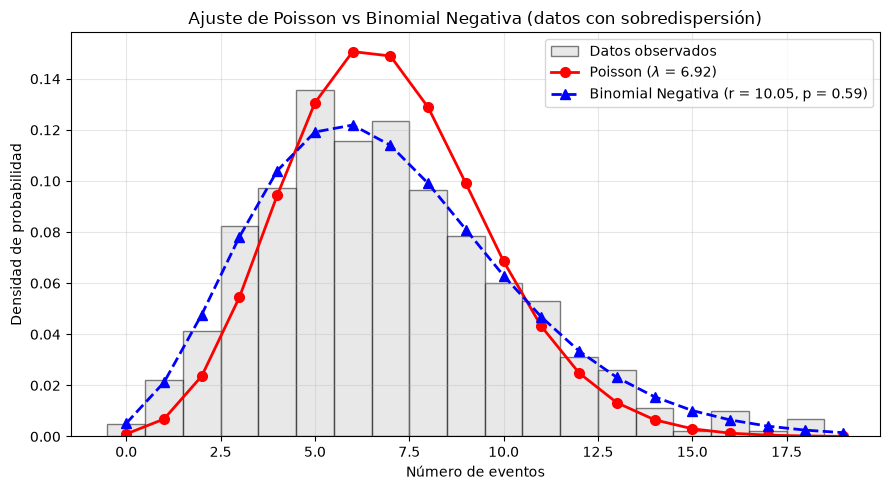
\includegraphics[height=7cm,keepaspectratio=true]{./pe/distDataScience.png}
 % distDataScience.png: 0x0 pixel, 300dpi, 0.00x0.00 cm, bb=
 \caption{Comparison of Poisson vs. Negative Binomial fit for overdispersed data}
 \label{fig:2.10.10}
\end{figure}

\begin{observacion}
	In practice, the choice of distribution depends on both the nature of the phenomenon being modeled and the statistical properties of the observed data. Tools such as the likelihood function, Akaike Information Criterion (AIC), and cross-validation allow us to compare different models and choose the most appropriate one.
\end{observacion}
